\documentclass[border=10pt]{standalone}

\usepackage{tikz}
\usepackage{tikzsymbols}
\usetikzlibrary{calc,patterns,shapes.geometric}

\def\centerarc[#1](#2)(#3:#4:#5){\draw[#1] ($(#2)+({#5*cos(#3)},{#5*sin(#3)})$) arc (#3:#4:#5);}

\begin{document}
	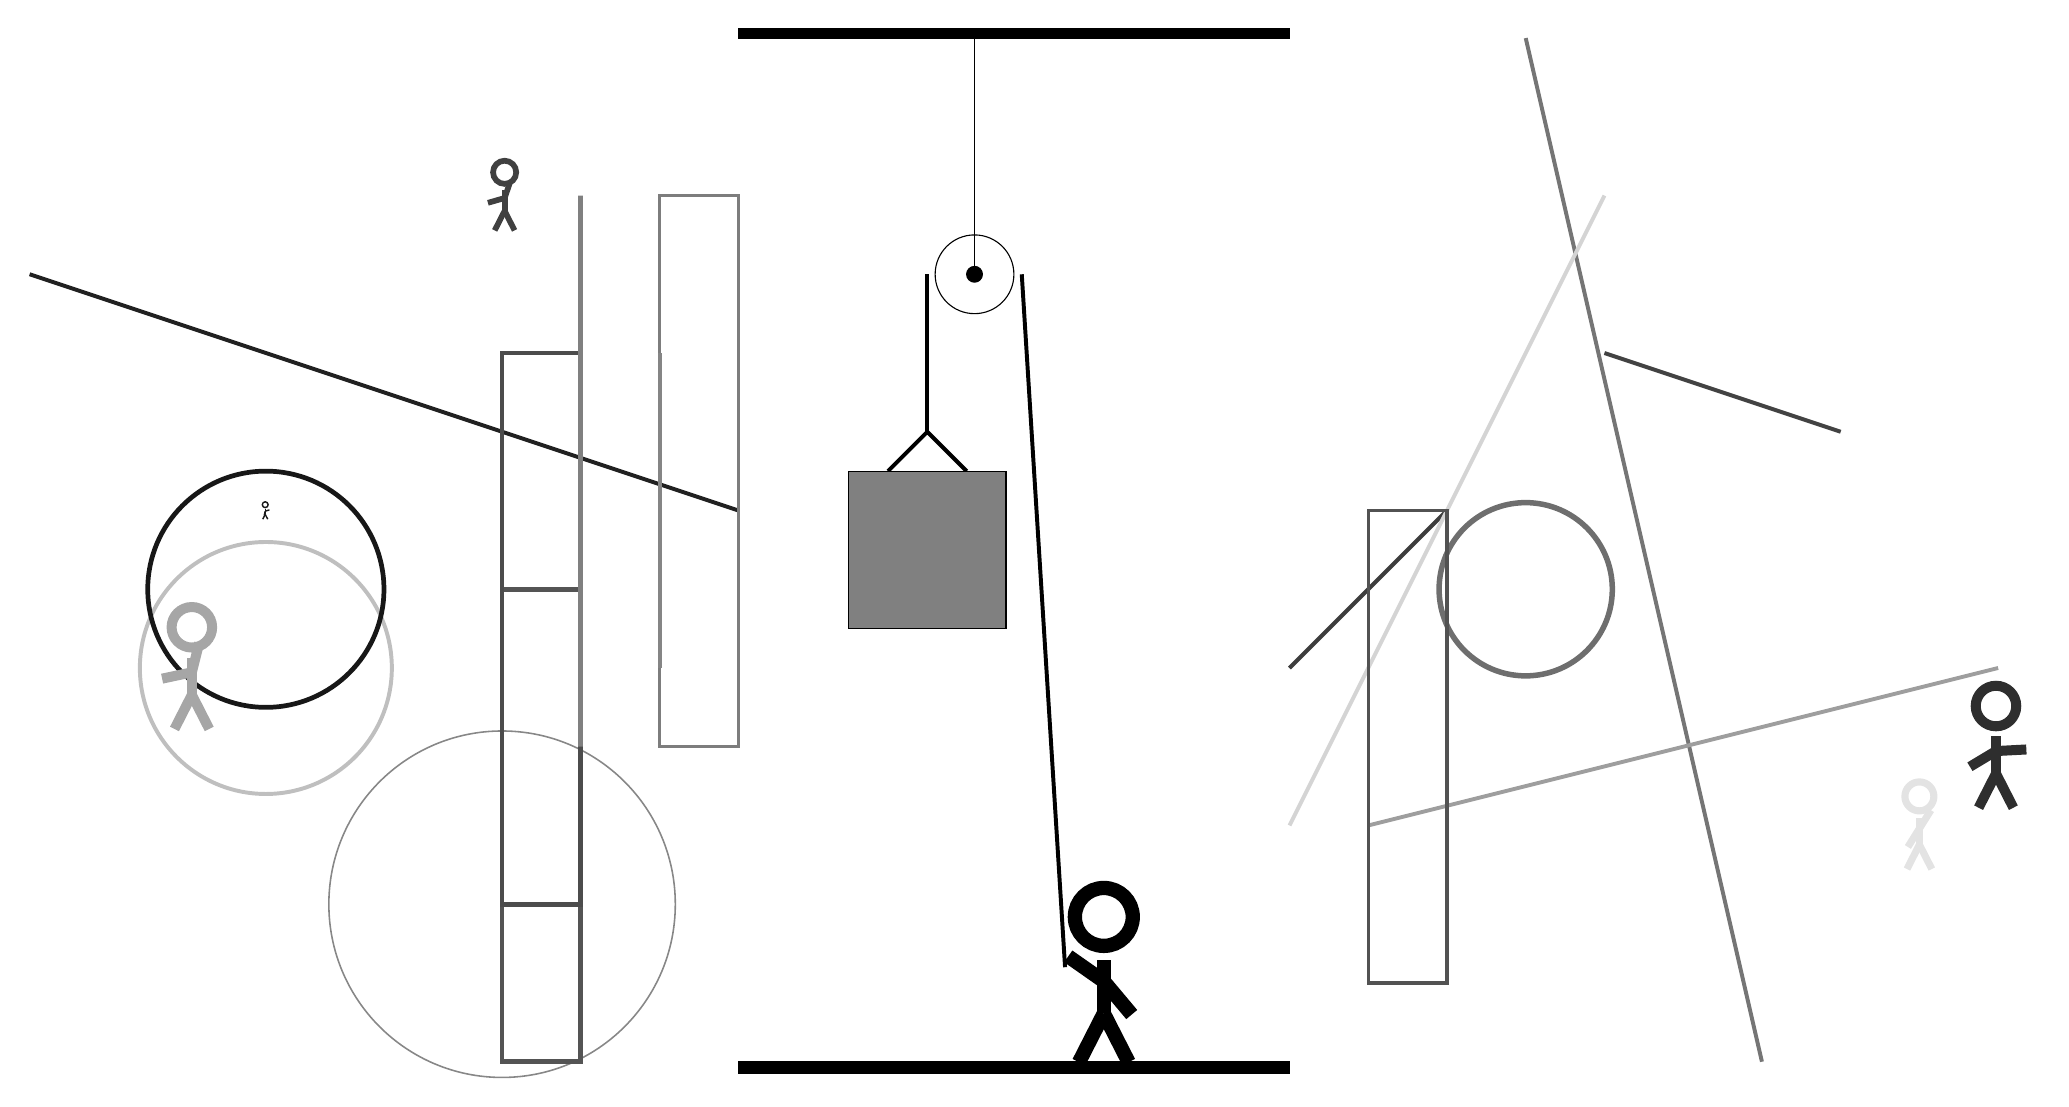
\begin{tikzpicture}
		%%%%% START %%%%%
		
		\draw[fill=black] (-2, 10) rectangle (5, 10.125);
		
		\draw (1, 7) circle (0.5);
		\draw[fill=black] (1, 7) circle (0.1);
		\draw (1, 10) -- (1, 7);
		
		\draw[line width=0.5mm] (-0.1, 4.5) -- (0.4, 5.0) -- (0.9, 4.5);
		\draw[fill=black!50] (-0.6, 4.5) rectangle (1.4, 2.5);
		
		\draw[line width=0.5mm] (0.4, 7) -- (0.4, 5.0);
		\centerarc[line width=0.5mm](1, 7)(0:180:0.6);
		\draw[line width=0.5mm](1.6, 7) -- (2.15, -1.8);
		
		\draw[line width=0.5mm, color=black!74](9, 6) -- (12, 5);
		
		\draw [line width=0.5mm, color=black!25](-8, 2) circle (1.6);
		\draw [line width=0.2mm, color=black!47](-5, -1) circle (2.2);
		\node[line width=0.6mm, color=black!75] at (-5, 8) {\Strichmaxerl[4][16][71]};
		\node[line width=0.2mm, color=black!90] at (-8, 4) {\Strichmaxerl[1][77][16]};
		
		\draw[line width=0.5mm, color=black!54](8, 10) -- (11, -3);
		
		\draw[line width=0.4mm, color=black!38] (-4, 2) rectangle (-4, 6);
		\draw[line width=0.5mm, color=black!76](5, 2) -- (7, 4);
		\draw [line width=0.7mm, color=black!57](8, 3) circle (1.1);
		
		\node[line width=0.2mm, color=black!82] at (14, 1) {\Strichmaxerl[7][31][3]};
		\draw[line width=0.5mm, color=black!87](-2, 4) -- (-11, 7);
		\draw[line width=0.6mm, color=black!67] (-4, 3) rectangle (-5, -3);
		\draw[line width=0.5mm, color=black!17](5, 0) -- (9, 8);
		\draw[line width=0.4mm, color=black!51] (-3, 1) rectangle (-2, 8);
		\draw[line width=0.5mm, color=black!38](6, 0) -- (14, 2);
		\draw [line width=0.6mm, color=black!91](-8, 3) circle (1.5);
		\draw[line width=0.4mm, color=black!68] (6, 4) rectangle (7, -2);
		\draw[line width=0.6mm, color=black!70] (-4, 6) rectangle (-5, -1);
		\draw[line width=0.6mm, color=black!50] (-4, 8) rectangle (-4, 1);
		\node[line width=0.2mm, color=black!11] at (13, 0) {\Strichmaxerl[5][58][58]};
		\draw[line width=0.5mm, color=black!48](-3, 6) -- (-3, 2);
		
		\node[line width=0.4mm, color=black!35] at (-9, 2) {\Strichmaxerl[7][12][76]};
		
		
		\node at (2.6, -1.9) {\Strichmaxerl[10][-35][-50]};
		
		\draw[fill=black] (-2, -3) rectangle (5, -3.15);
		
		%%%%% END %%%%%
	\end{tikzpicture}
\end{document}